\chapter{Основные сведения о курсорах, наборах данных и временных таблицах}
\section{Сравнительная оценка использования решений на основе курсоров/итераций и решений на основе наборов данных}


\begin{figure}[h!]
	\begin{center}
		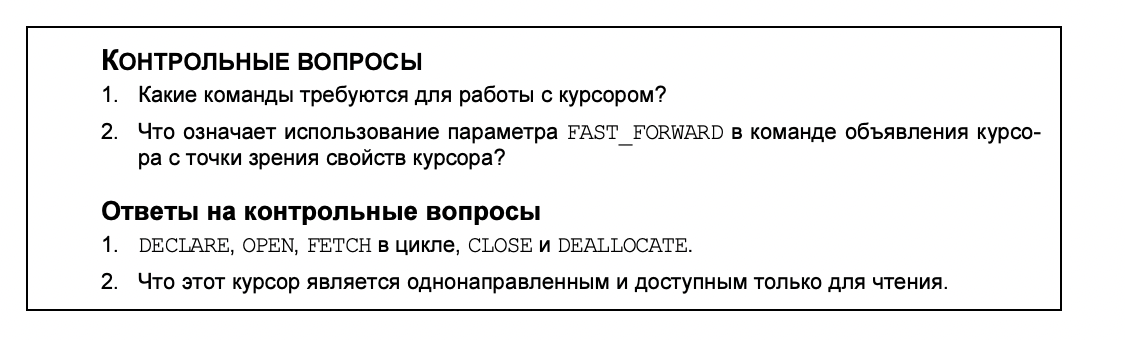
\includegraphics[width=0.9\textwidth]{img/control44.png}
	\end{center}
	\captionsetup{justification=centering}
\end{figure}


\subsection*{Резюме занятия}
\begin{itemize}
	\item Вы можете использовать один из двух основных подходов к решению связанных
	с запросами задач; один — использование решения на основе наборов данных,
	другой — использование итерационных решений. 
	\item Решения на основе наборов используют SQL-запросы, которые следуют принципам реляционной модели. Они взаимодействуют с входными таблицами (наборами) как с единым целым, в отличие от построчного взаимодействия. Они
	также не ожидают, что данные будут приниматься или возвращаться в определенном порядке. 
	\item Некоторые задачи должны решаться с помощью итерационных решений, к ним
	относятся задачи управления, которые должны выполняться для каждого объекта, или хранимые процедуры, которые нужно выполнять в таблице построчно. 
	\item Что касается связанных с запросами задач, обычно по умолчанию рекомендуется использовать решения на основе наборов, а итерационные решения применять только в исключительных случаях. 
\end{itemize}

\subsection*{Закрепление материала}

\begin{figure}[h!]
	\begin{center}
		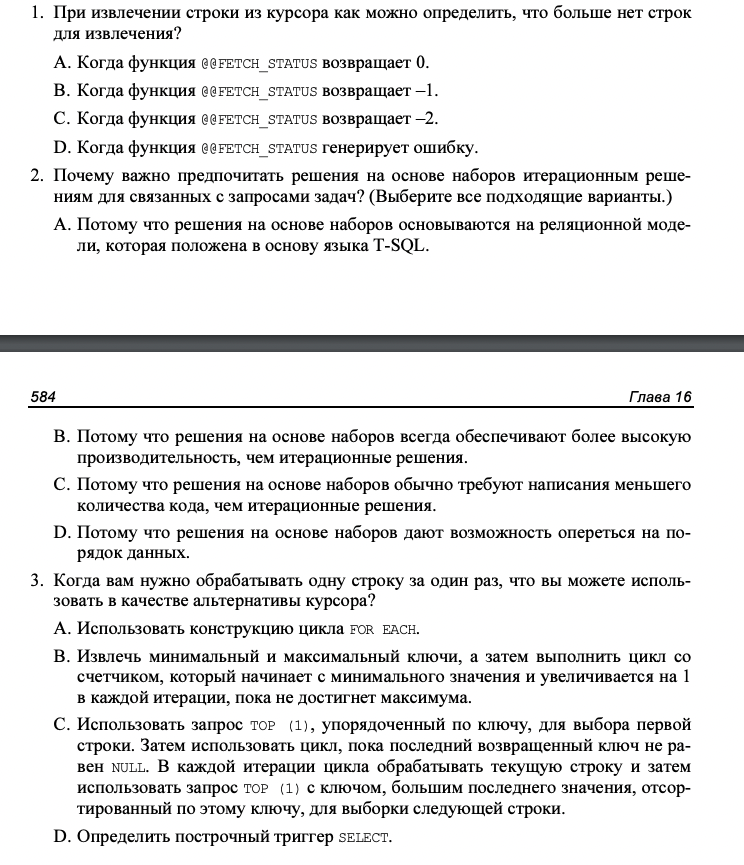
\includegraphics[width=0.8\textwidth]{img/zakrep46.png}
	\end{center}
	\captionsetup{justification=centering}
\end{figure}
\newpage

\subsection*{Ответы}

\begin{figure}[h!]
	\begin{center}
		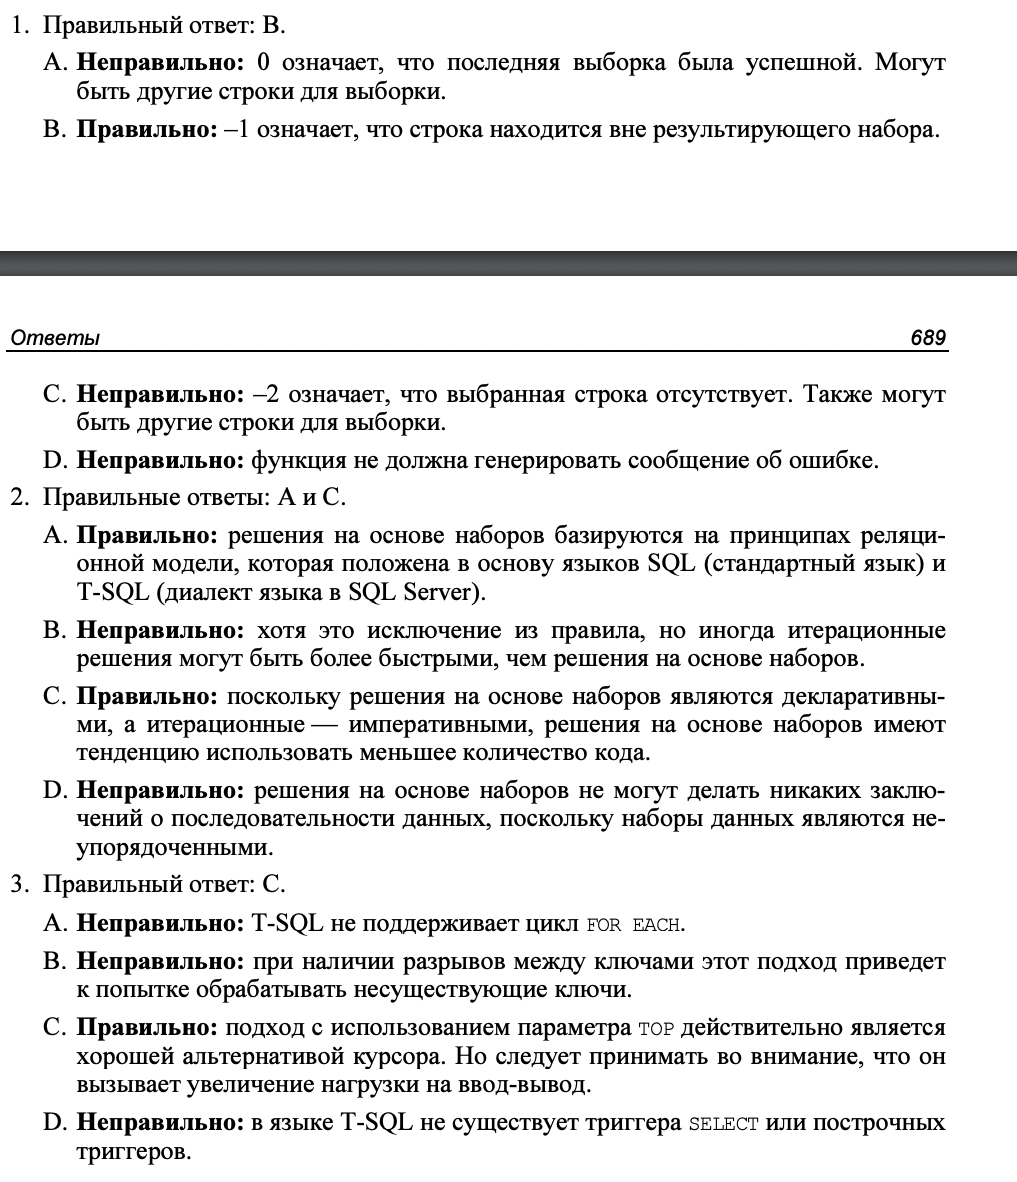
\includegraphics[width=0.9\textwidth]{img/ans46.png}
	\end{center}
	\captionsetup{justification=centering}
\end{figure}
\clearpage



\section{Сравнение использования временных таблиц и табличных переменных }

Табличные
переменные хорошо использовать в двух общих случаях. Один — когда объем данных настолько маленький, как страница или две, что эффективность плана
не имеет значения. Другой случай — когда план очень простой. Простой
план означает, что существует только один разумный план, и оптимизатору фактически не нужны гистограммы для принятия решения.

\begin{figure}[h!]
	\begin{center}
		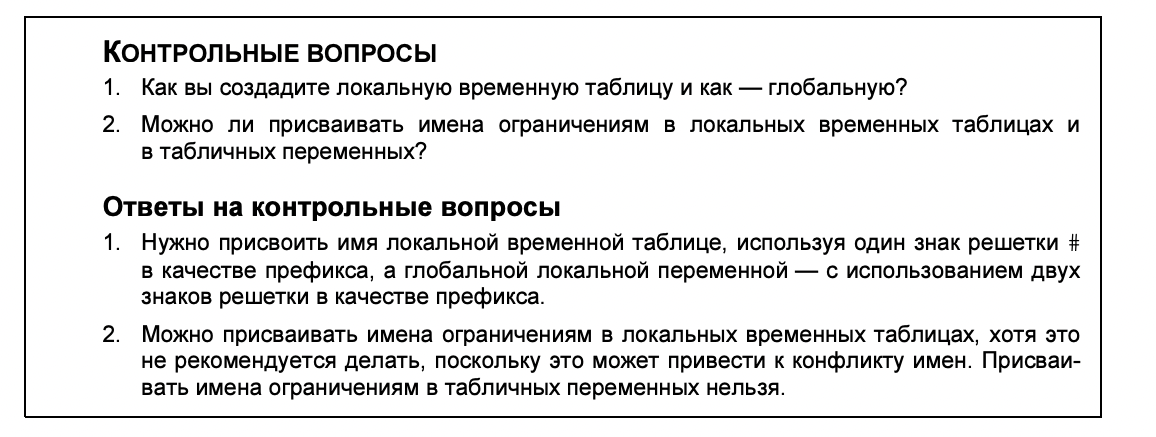
\includegraphics[width=0.9\textwidth]{img/control45.png}
	\end{center}
	\captionsetup{justification=centering}
\end{figure}


\subsection*{Резюме занятия}
\begin{itemize}
	\item Вы можете использовать временные таблицы и табличные переменные, когда
	вам нужно временно сохранить данные, такие как промежуточный результирующий набор запроса. 
	\item Временные таблицы и табличные переменные имеют множество различий,
	включая область действия, язык DDL и индексирование, взаимодействие с транзакциями и статистику распространения. 
	\item Локальные временные таблицы видны уровню, который их создал, всем пакетам
	этого уровня, а также внутренним и уровням в стеке вызовов. Табличные переменные видны только пакету, который их объявил. 
	\item Можно применять язык DDL к временной таблице после ее создания, включая
	создание индексов и другие изменения DDL. Нельзя применять изменения DDL
	к табличной переменной после ее объявления. В табличной переменной можно
	создавать индексы косвенным образом посредством ограничений первичного
	ключа и уникальности. 
	\item Изменения, примененные к временной таблице в транзакции, отменяются при
	откате этой транзакции. Изменения, примененные к табличной переменной, не
	отменяются при откате транзакции. 
	\item SQL Server поддерживает статистику распространения на временных таблицах,
	но не на табличных переменных. В результате, планы запросов, использующих
	временные таблицы, более оптимальны, чем планы с использованием табличных
	переменных. 
\end{itemize}


\subsection*{Закрепление материала}

\begin{figure}[h!]
	\begin{center}
		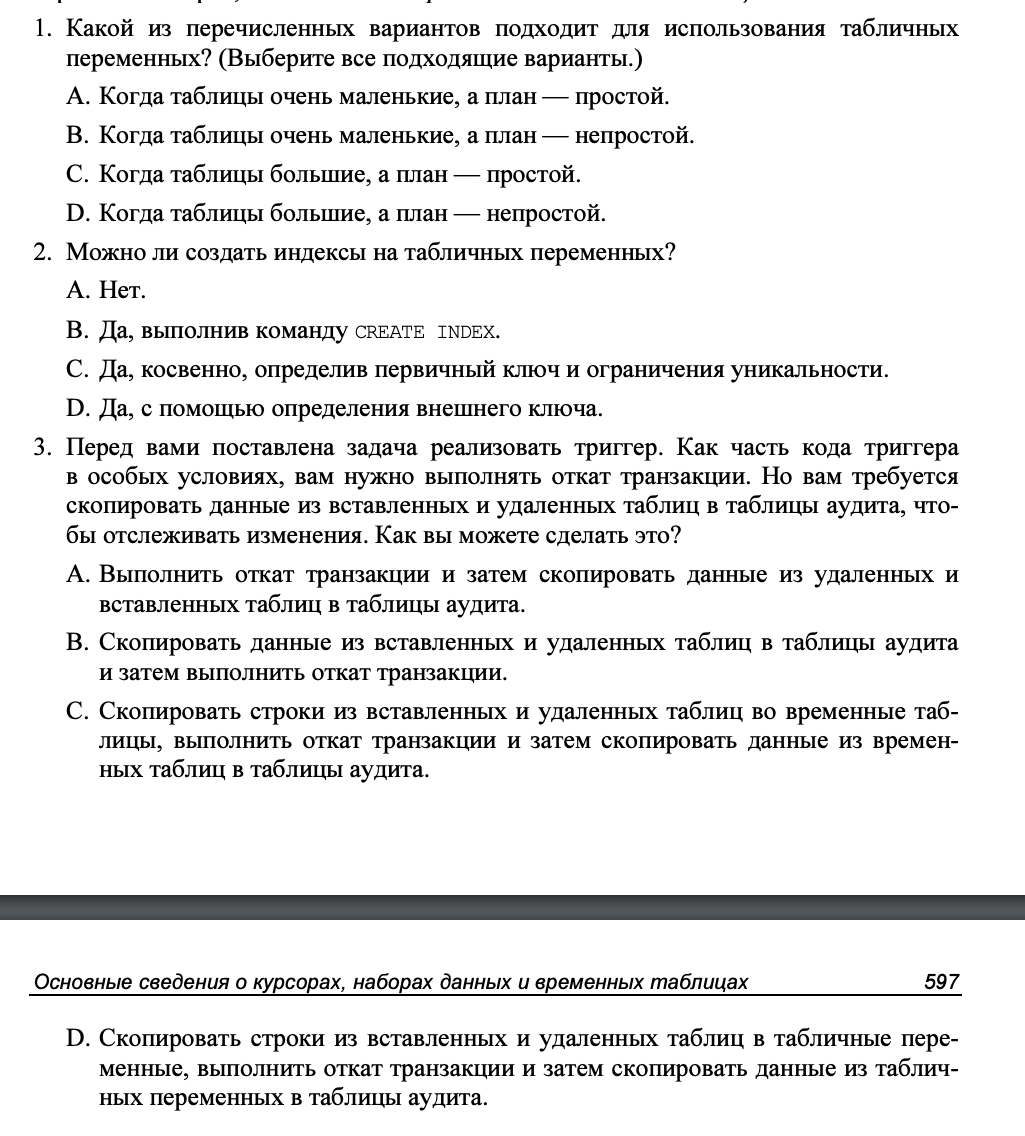
\includegraphics[width=0.7\textwidth]{img/zakrep47.png}
	\end{center}
	\captionsetup{justification=centering}
\end{figure}
\clearpage	

\subsection*{Ответы}

\begin{figure}[h!]
	\begin{center}
		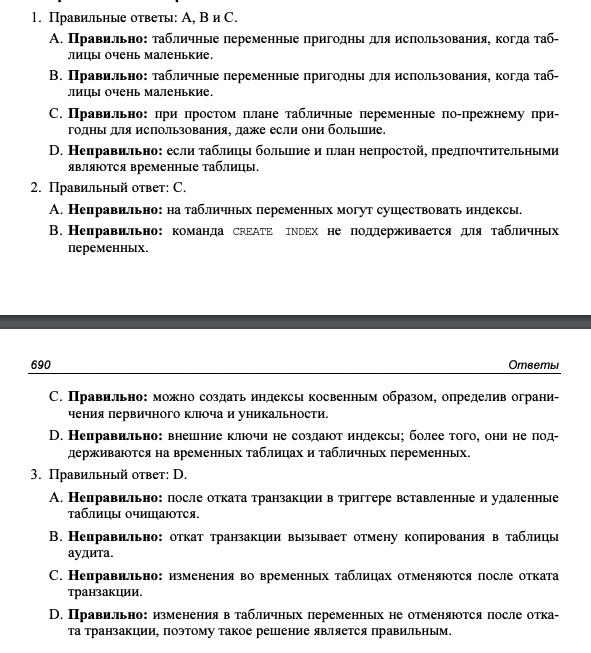
\includegraphics[width=0.9\textwidth]{img/ans47.png}
	\end{center}
	\captionsetup{justification=centering}
\end{figure}

\newpage
\subsection*{Упражнения}

\begin{figure}[h!]
	\begin{center}
		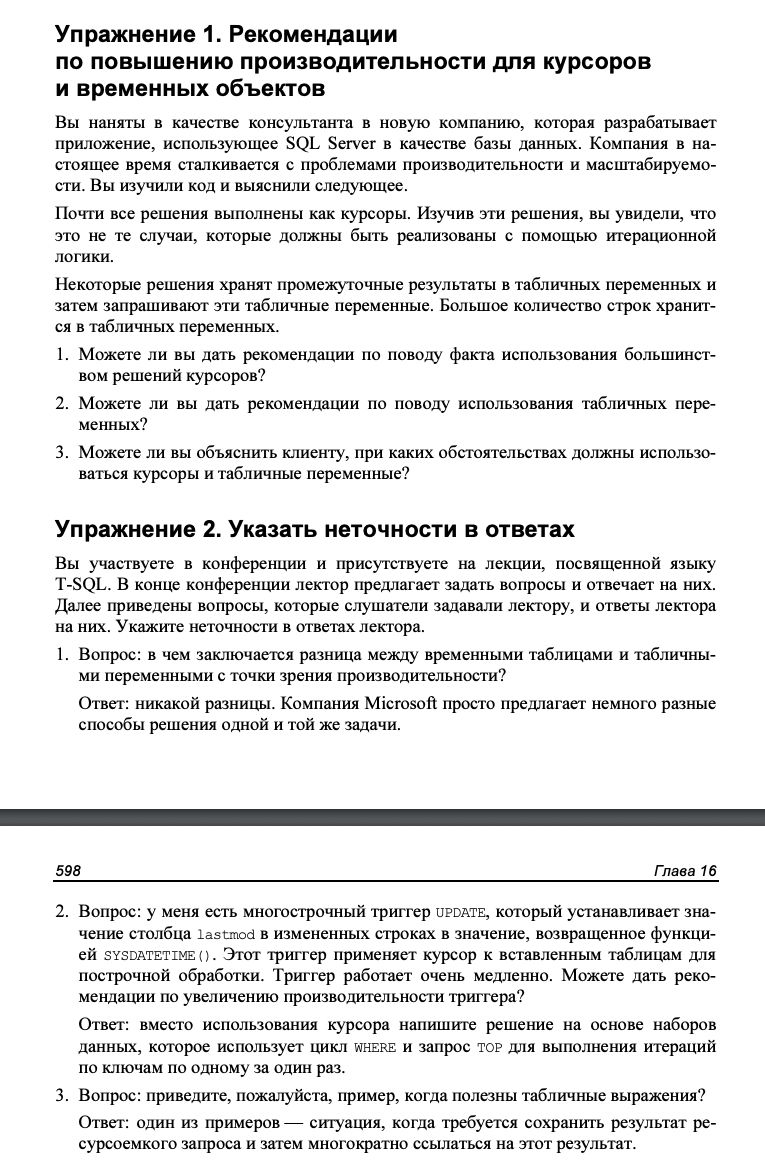
\includegraphics[width=0.7\textwidth]{img/ex20.png}
	\end{center}
	\captionsetup{justification=centering}
\end{figure}


\newpage
\subsection*{Ответы}

\begin{figure}[h!]
	\begin{center}
		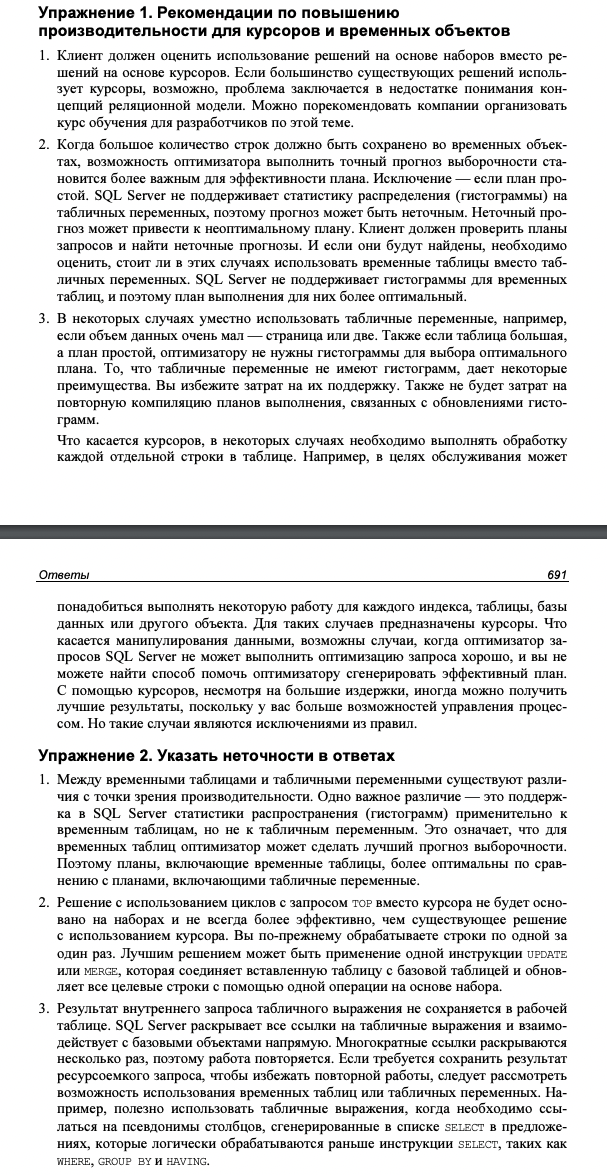
\includegraphics[width=0.6\textwidth]{img/eans20.png}
	\end{center}
	\captionsetup{justification=centering}
\end{figure}